\chapter{Special relativity}
\label{chap:relativity}
This chapter gives a basic outline of the theory of special relativity. It is by no means meant to be a comprehensive overview, for which many other excellent resources exist such as \citet{Misner1970}, \citet{Taylor1992}, \citet{Landau1971}, or \citet{Penrose1978} for a shorter, less technical introduction. Instead, the goal of this section is to give a physical context for the concept of Lorentz geometry and the associated Lorentz space and metric, as well as their connection with hyperbolic geometry discussed in \cref{chap:relativity}, and Möbius transforms which will be introduced in \cref{chap:moebius_transforms}.

First, \cref{sec:time_relative} introduces the relativity of time and the concept of spacetime. Consequently, \cref{sec:spacetime_intervals} proceeds with the definition of spacetime intervals, the analog of distance in spacetime. This can be generalized to the notion of a Lorentzian vector space, the subject of \cref{sec:lorentz_transformations}. Finally, \cref{sec:lorentz_transformations} discusses the transformations of spacetime that preserve the spacetime interval: the Lorentz transformations.

\section{Time as a relative concept}
\label{sec:time_relative}
Before the advent of the theory of special relativity, developed by i.a. Poincaré, Minkowski, Lorentz and Einstein, so-called `Galilean relativity' was the norm. Galilean relativity entails the definition of Galilean transformations which, link reference frames that move relative to each other at a constant linear velocity. The laws of physics should be invariant between these inertial reference frames. However, a problem presented itself in the form of the famous Maxwell equations that pose the governing laws in electromagnetism. A consequence from Maxwell's laws is the finite propagation speed of light, and therefore all possible interactions between particles in the universe. It is not hard to imagine that the Galilean invariance breaks down as a result of the introduction of a `special' speed --- indeed, the Galilean transform proclaims a complete independence between the physical laws and the constant velocity of the frame in which they are applied. But, as a direct consequence from Maxwell's equations, the laws of physics in a moving reference frame \emph{will} depend on the velocity of that particular reference frame: a major inconsistency with the traditional train of thought.

The new principle of relativity that brought reconciliation with Maxwell's ideas not only required space to be relative (i.e. dependent on a frame of reference), but also views \emph{time as a relative concept} whereas, it had always been assumed to be absolute in classical mechanics. As such, the notion of time is dependent on the choice of reference frame too. This has the immediate consequence that the traditional three-dimensional setting of classical mechanics (often with Cartesian coordinates \lsymb{$x, y, z$}{Spatial coordinates of spacetime}) will not suffice for the description of special relativity: a fourth coordinate for time is indispensable to incorporate the relativity of time. Points in the four-dimensional \emph{spacetime} are called \emph{world points}, their associated trajectories are \emph{world lines} \cite{Landau1971}.
\index{world line}
\index{world point}
\index{Galilean relativity}
\index{speed of light}

\section{Spacetime intervals}
\label{sec:spacetime_intervals}
Overwhelming experimental evidence has pointed out that the propagation of light is completely independent of its direction. This can be encapsulated in spacetime by means of \emph{spacetime intervals} which provide a notion of distance between two world points. If a signal travels at the speed of light \lsymb{$c$}{Speed of light}, the distance between two world points along its trajectory should be zero. The spatial distance squared between two points is equal to
\index{spacetime interval}
\[
    \qty(x_2 - x_1)^2 + \qty(y_2 - y_1)^2 + \qty(z_2 - z_1)^2,
\]
whereas the distance squared covered by a signal traveling at the speed of light is equal to 
\[c^2(t_2 - t_1)^2. \]
Therefore, the spacetime interval \lsymb{$s_{12}$}{Spacetime interval} between two world points is:
\[
    s_{12} = \sqrt{c^2(t_2 - t_1)^2 - \qty(x_2 - x_1)^2 - \qty(y_2 - y_1)^2 - \qty(z_2 - z_1)^2},
\]
which will amount to zero for the world lines corresponding to a signal traveling at the speed of light. For an infinitesimal distance \(\dd{s}\), the spacetime interval can be expressed as
\[ \dd{s}^2 = c^2 \dd{t}^2 - \dd{x}^2 - \dd{y}^2 - \dd{z}^2.\]
The spacetime interval is the same in any inertial reference frame. This is the mathematical translation of the invariance of the speed of light in the universe \cite{Landau1971}. Based on the sign of the spacetime interval, three classes can be distinguished:
\begin{itemize}
    \item If \(s_{12}^2 > 0\), the interval is \emph{timelike}, and there exists a frame of reference in which both events occurred \emph{at the same location} in space, they are simply separated by the passage of time \(\displaystyle t_{12} = \frac{s_{12}}{c}\). 
    \item When \(s_{12}^2 < 0\), the interval is \emph{spacelike}, and the events are `too far apart' to reach within the limits of the speed of light --- the events must therefore be at different locations (absolutely remote), and there exists a reference frame in which the events occur \emph{simultaneously} \(l_{12} = \ii s_{12}\), where \lsymb{$\ii$}{Imaginary unit} is the imaginary unit.
    \item Intervals for which \(s_{12}^2 = 0\) are called \emph{lightlike}, because only light (or anything traveling at the speed of light) can travel between these events.
\end{itemize}
\index{lightlike}
\index{spacelike}
\index{timelike}
This begs the question what the actual time is that an observer would experience in uniform motion, i.e. what difference in time is displayed by clocks that have been traveling at different velocities. The time experienced by an observer is called \emph{proper time}, and it can be computed by evaluating the following path integral:
\index{proper!time}
\begin{equation}
    t'_2 - t'_1 = \int^{t_2}_{t_1} \dd{t} \sqrt{1 - \qty(\frac{v}{c})^2}.
    \label{eq:proper_time}
\end{equation}
Clearly, if the velocity \lsymb{$v$}{velocity} makes up a larger fraction of the speed of light, the proper time is lower; that is, moving clocks run slower than a clock at rest (hypothetical clocks traveling at the speed of light do not register the passage of time whatsoever).

\section{Lorentzian vector spaces}
\label{sec:lorentz_metric}
The concept of the spacetime interval introduced in the previous section gives rise to a different notion of `distance' in four-dimensional spacetime. This distance is different from the traditional Euclidean distance: it is a \emph{Lorentzian} distance. This different notion of distance is captured by the definition of the \emph{Lorentz(ian) product}\footnote{In literature (both physics and mathematics) many variations on the so-called `metric signature' of the Lorentz product make their appearance. In terms of \(\real^4\), these variations come down to \((+,-,-,-)\), \((-,-,-,+)\), \((-,+,+,+)\) and \((+,+,+,-)\), where the first one coincides with the definition used here, in accordance with the magnificent work of \citet{Landau1971}. Luckily, this is just a matter of convention and its influence on the mathematical machinery at hand is limited to the switching of some signs.}.

\begin{thmblock}{Lorentz product}
    Let \(\vec{u}, \vec{w}\) be vectors in \lsymb{\(\real^n\)}{Real $n$-dimensional vector space}. The \emph{Lorentzian inner product} \others{$\bullet$}{Lorentzian inner product} of \(\vec{u}\) and \(\vec{w}\) is defined to be the real number
    \begin{equation}
        \vec{u} \bullet \vec{w} = u_1w_1 - u_2w_2 - \ldots - u_nw_n.
        \label{eq:lorentz_product}
    \end{equation}
\end{thmblock}
%The Lorentz product is an inner product, which means that it takes two elements from a vector space and returns a scalar value, while satisfying two (or three) conditions: (i) bilinearity, (ii) symmetry, and (iii) nondegeneracy 
The Lorentz product resembles the `normal'  inner product, with the exception of the minus signs before every but the first term. These minus signs are the reason why the Lorentz product is an indefinite product; that is, it fails to be positive definite. An inner product satisfies (i) bilinearity, (ii) symmetry, and (iii) positive definiteness. As discussed in the previous section, the inner product of a spacelike vector with itself will \emph{not} return a positive number;  a lightlike vector will produce 0. As such, the Lorentz product is indefinite, which is why it is called a \emph{pseudo-inner product} \cite{Ratcliffe2019,Schuller2014}. The weaker condition that is imposed for pseudo-inner products asserts that it must be nondegenerate, which means that there exists no non-zero vector for which its inner product with any other vector is zero.
\index{Lorentz!-ian vector space}
\index{Lorentz! inner product}

Based on the Lorentz inner product it is natural to define also a corresponding \emph{Lorentzian norm} \others{\(\lnorm{\cdot}\)}{Lorentzian norm}:
    \[
     \lnorm{\vec{u}} = \qty(\vec{u}\bullet\vec{u})^\frac{1}{2}.
\]
Because the Lorentz product is not positive definite but indefinite, the result of \(\vec{u}\bullet\vec{u}\) is not guaranteed to be a positive number. As such, \(\lnorm{\vec{u}} \in \) \lsymb{\(\complex\)}{Complex numbers}, in stark contrast with the familiar Euclidean norm which \emph{is} positive definite and will therefore always return a non-negative real number.

The norm provides a notion of length for a vector. Based on this length, a \emph{metric} yields a distance between two points, i.e. the distance between \(\vec{u}\) and \(\vec{w}\) is equal to:
\index{Lorentz!norm}
\index{pseudo-Euclidean space}
\[
     d_L(\vec{u}, \vec{w}) \triangleq \lnorm{\vec{u} - \vec{w}}
\] 
Because the norm is not positive definite but `only' nondegenerate, it is called a \emph{pseudo-Euclidean metric}, and the vector space it is associated with a \emph{pseudo-Euclidean space}. A vector space equipped with this pseudometric (in more general terms, a bilinear nondegenerate form) is called a Lorentz space. The particular case for \(\real^4\) sets the stage for the theory of special relativity (with one `special' dimension for time and three spatial dimensions) and is called the Minkowski space, after the German physicist Hermann Minkowski \cite{Catoni2008}. Elements of the Minkowski space are denoted by \emph{four-vectors}. Often, Lorentzian spaces are denoted in short by \lsymb{$\real^{p,q}$}{Lorentzian vector space} where the combination $p,q$ indicates the metric signature. $p$ and $q$ respectively denote the number of plus and minus signs in the Lorentzian product. The total dimension of the space is then $p + q$. As such, the Minkowski space is denoted by $\real^{1,3}$. However, there are other Lorentzian spaces as well; in \cref{ssec:hyperboloid} the discussion involves a three-dimensional Lorentzian space (with two spatial directions and one `time' dimension) $\real^{1,2}$. Likewise, concepts in spatial relativity are usually illustrated using the Lorentz-Minkowski plane, which is basically a two-dimensional representation of spacetime referred to as $\real^{1,1}$. This Lorentzian space will play an important role in \cref{chap:finance_rotation}.
%Sometimes the two-dimensional plane that is discovered here is also called the Minkowski plane, because this is what he used to explain his ideas, being unable to draw anything like four-dimensional space. However, this text will adhere to the more mathematically inclined tradition and call it `Lorentz(ian) space' which applies to any dimension larger than one \cite{Ratcliffe2019}. The theory of special relativity, and especially the role of the Lorentz metric will be discussed in \cref{chap:relativity}.
\index{four-vectors}
\index{Lorentz-Minkowski plane}

The sign of the Lorentz norm gives rise to an equivalence relation\footnote{An equivalence relation \others{$\sim$}{Equivalence relation} is a binary relation that is symmetric, reflexive and transitive.}  \(\sim_L\) defined to be:
$$\vec{u} \sim_L \vec{w} \iff \sgn{\norm{\vec{u}}}_L = \sgn{\norm{\vec{w}}}_L.$$
Therefore, the quotient set of all the points in the plane \(\real\,\backslash\sim_L\) contains three elements \(\qty{-1, 0, 1}\), these equivalence classes are given the respective names spacelike, lightlike and timelike, analogous to the terminology for the spacetime intervals from the previous section \cite{Landau1971}. The difference between timelike, spacelike and lightlike vectors is illustrated for the Lorentz-Minkowski plane in \cref{fig:lightlike_spacelike}.
\index{equivalence relation}

\begin{figure}[ht]
    \centering
    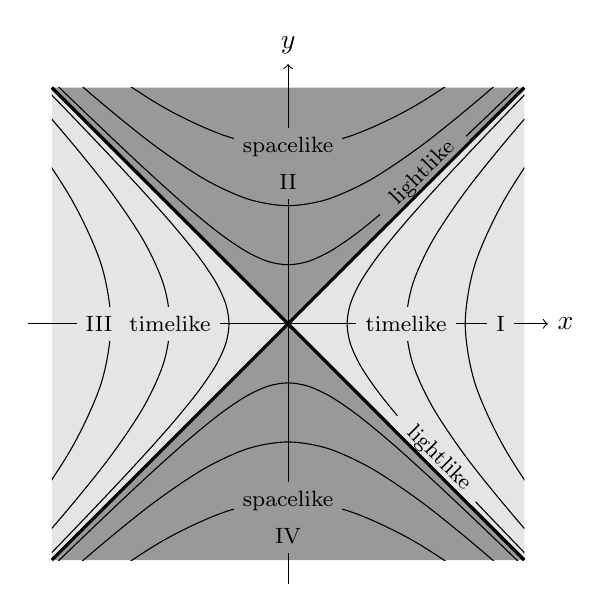
\begin{tikzpicture}[scale=1.5]
    
    \fill[fill=gray!20] (0,0) -- (2, 2) -- (2, -2) --cycle;
    \fill[fill=gray!20] (0,0) -- (-2, 2) -- (-2, -2) --cycle;
    
    \fill[fill=gray!80] (0,0) -- (-2, 2) -- (2, 2) --cycle;
    \fill[fill=gray!80] (0,0) -- (-2, -2) -- (2, -2) --cycle;
    
    \begin{scope}

        \clip (-2, -2) rectangle (2, 2);
        \foreach \K in {0.5, 1, 1.5} {
            \draw[smooth, domain=-4:4, variable=\t] plot ({\K*cosh(\t)}, {\K*sinh(\t)});
            \draw[smooth, domain=-4:4, variable=\t] plot ({-\K*cosh(\t)}, {-\K*sinh(\t)});
            
            \draw[smooth, domain=-4:4, variable=\t] plot ({\K*sinh(\t)}, {\K*cosh(\t)});
            \draw[smooth, domain=-4:4, variable=\t] plot ({-\K*sinh(\t)}, {-\K*cosh(\t)});
        }
    \end{scope}
    
    \draw[very thick] (-2, -2) -- (2, 2) node[above,pos=0.8, sloped,fill=gray!80,inner sep=0cm] { \ \rotatebox[origin=c]{90}{$\Lsh$} \footnotesize{lightlike} \rotatebox[origin=c]{270}{$\Rsh$} \ };
    \draw[very thick] (2, -2) -- (-2, 2) node[above,pos=0.2, sloped,fill=gray!20,inner sep=0cm] { \ \rotatebox[origin=c]{90}{$\Lsh$} \footnotesize{lightlike} \rotatebox[origin=c]{270}{$\Rsh$} \ };
    
    \draw[->] (-2.2, 0) -- (2.2, 0) node[right] {$x$};
    \draw[->] (0, -2.2) -- (0, 2.2) node[above] {$y$};
    
    
    
    \node[fill=gray!80] at (0, 1.5) {\footnotesize{spacelike}};
    \node[fill=gray!80] at (0, 1.2) {\footnotesize{II}};
    \node[fill=gray!80] at (0, -1.5) {\footnotesize{spacelike}};
    \node[fill=gray!80] at (0, -1.8) {\footnotesize{IV}};
    fill=w
    \node[fill=gray!20] at (1, 0) {\footnotesize{timelike}};
    \node[fill=gray!20] at (1.8, 0) {\footnotesize{I}};
    \node[fill=gray!20] at (-1, 0) {\footnotesize{timelike}};
    \node[fill=gray!20] at (-1.6, 0) {\footnotesize{III}};
                
    % TODO: Add some hyperbolas
    
\end{tikzpicture}
    \caption{Overview of the three `types' of vectors in the Lorentz-Minkowski plane: spacelike (\(\lnorm{\vec{u}} < 0\)), lightlike (\(\lnorm{\vec{u}} = 0\)) and timelike (\(\lnorm{\vec{u}} > 0\)). The lines \(ct = x\) and \(ct = -x\) containing all the lightlike vectors form the so-called light cone or null cone. Points with vectors with identical length trace out hyperbolae, as they obey the equation $c^2t^2 - x^2 = K^2$.} %The hyperbola of in the spacelike region (dark gray) obey the equation \(ct^2 - x^2 = K^2\), they will be referred to the hyperbolic branches II (\(y > 0\)) and IV (\(y < 0\)). In contrast, the timelike hyperbolic branches with equation \(x^2 - y^2 = K^2\) (light gray region) are referred to as I (\(x > 0\)) and III (\(x < 0\)).}
    \label{fig:lightlike_spacelike}
\end{figure}
\index{light cone}
%The financial interpretation of the lightlike vectors is all the capital-yield combinations that are attainable, which is why spacelike vectors are fictitious in this regard if only the action of compound interest is considered. However, when one looks at velocities in this vector space; i.e. how fast a position vector is changing, the velocity vector can be spacelike due to capital injections that change the `arm' of the investment. 

%Instead of the usual three-vectors that are common in classical mechanics, points in spacetime may be regarded as elements in a four-dimensional vector space instead:
%\begin{equation}
%    A^0 = ct\qquad A^1 = x \qquad A^2 = y \qquad A^3 = z;
%    \label{eq:four-vector}
%\end{equation}
%where the superscript indices indicate \emph{contravariant} (vector) components. However, the 
%These can be converted to covariant indices by virtue of the metric tensor \tens{g}
%\index{metric tensor}
%\begin{equation}
%    g_{ij} = g^{ij} = \mqty(\dmat[0]{1, -1, -1, -1}).
%    \label{eq:lorentz_metric}
%\end{equation}
%Using \tens{g}, indices can then be lowered (or raised) like so
%\[ A^0 = A_0\qquad A^1 = -A_1 \qquad A^2 = -A_2 \qquad A^3 = -A_3; \]
%such that the spacetime interval may be expressed in tensor notation (observing the Einstein summation convention) as
%\[ s^2 = A^i A_i = c^2t^2 - x^2 - y^2 - z^2.\]

\section{Lorentz transformations}
\label{sec:lorentz_transformations}
As mentioned, special relativity corrects for a flaw of the Galilean transforms, which represent the classical view of inertial reference systems. For example, if one coordinate system moves at constant velocity \lsymb{$V$}{Velocity (between reference frames)} with respect to the other in \(x\)-direction (the coordinate directions are assumed to coincide for simplicity), the Galilean transform takes the form:
\begin{equation}
    x = x' + Vt, \quad y = y', \quad z = z',\quad t = t'.
    \label{eq:galilean_transform}
\end{equation}
The statement \(t = t'\) encodes the traditional assumption in mechanics that time has an absolute character. Of course, it is precisely this statement that is refuted by special relativity. As such, one could devise a new type of transformation that takes this (and the invariance of spacetime intervals between events, as discussed in the previous section) into account. These transformations are called \emph{Lorentz transformations}. 

As described by \citet{Landau1971}, these transformations comprise the rotations in four-dimensional space; since there are six ways to pick a plane (or two coordinates) from a set of four axes, every rotation in four-space can be decomposed into six successive rotations. Of these six rotations, three are purely spatial: they are the familiar rotations that can be parameterized by e.g. Euler angles or quaternions. On the other hand, the three other rotations involve time as well, and they are of a different nature. Whereas the spatial rotations are circular, the time-rotations are hyperbolic rotations (they are represented by hyperbolic functions rather than trigonometric functions). For example, a rotation in the \(tx\)-plane would take the following form:
\begin{equation}
    x = ct'\sinh(\zeta)\qquad ct = ct'\cosh(\zeta);
    \label{eq:lorentz_transform_hyp}
\end{equation}
\index{Lorentz!transformation}
or, using the fact that \(V = x/t\):
\begin{equation}
    x = \largefrac{x' + Vt'}{\sqrt{1 - \qty(\frac{V}{c})^2}} 
    \qquad t = \largefrac{t' + \frac{V}{c^2}x'}{\sqrt{1 - \qty(\frac{V}{c})^2}} \qquad y = y' \qquad z = z'.
    \label{eq:lorentz_transform_sqrt}
\end{equation}
This indicates that the hyperbolic (boost) angle \gsymb{\(\zeta\)}{Hyperbolic angle} can be written in terms of the velocity \(V\) of one frame with respect to the other frame:
\[ \tanh(\zeta) = \frac{V}{c}.\]
This implies that the argument of the hyperbolic rotation purely depends on the relative velocity between the two reference frames as a fraction of the speed of light. A few observations can be made based on these equations: 
\begin{itemize}
    \item Clearly, \(V\) cannot be larger than \(c\): there is no real \(\zeta\) for which this could be true. This again reaffirms the statement that there can be no motions with velocities larger than the speed of light.
    \item Secondly, the transform \cref{eq:lorentz_transform_sqrt} keeps \(c^2t^2 - x^2\) unaffected (\(z\) and \(y\) keep their value for obvious reasons); all points in the \(tx\)-plane that remain invariant under this type of transformations lie on the same hyperbola. %This underlines the connection with the capital-yield plane discussed in the previous sections: in that analogy, the accumulated interest corresponds to the Lorentz boost \(\zeta\).
    \item In the limit for \(c \to \infty\), the original Galilean transform is recovered; as such, the original laws still function as an approximation when \(V\) is of negligible size in comparison to \(c\).
    \item Due to the multiplication factor in the transform, two points and are closer (in the direction of $x$) together when traveling at speed than when they are at rest. A length measured in a rest frame is called \emph{proper}, and contracts when in measured a moving frame: this phenomenon is called \emph{Lorentz contraction} \index{Lorentz!contraction} \index{proper!length} \cite{Landau1971}.
    \index{Lorentz!boost}
    \item In contrast to Galilean transforms, Lorentz transforms are generally not commutative: just like regular three-dimensional rotations, they depend on the order in which they are applied.
\end{itemize}
\paragraph{Velocity transform} The Lorentz transform described by \cref{eq:lorentz_transform_hyp,eq:lorentz_transform_sqrt} shows how to transform coordinates from one frame to another. However, because the transform affects both \(x\) and \(t\), a velocity measured in the frame (not to be confused with the relative velocity between the frames \(V\)) \(\vec{v}\) with components will see not only its \(x\)-component affected, but the other two components \(v_x\) and \(v_z\) as well. The transformation of \(\vec{v}\) to \(\vec{v}'\) is: \cite{Landau1971}
\begin{equation}
    v_x = \largefrac{v_x' + V}{\sqrt{1 - \qty(\frac{V}{c})^2}}\qquad 
    v_y = \largefrac{v_y'\sqrt{1 - \qty(\frac{V}{c})^2}}{1 + v_x'
    \qty(\frac{V}{c})}\qquad
    v_z = \largefrac{v_z'\sqrt{1 - \qty(\frac{V}{c})^2}}{1 + v_x'\qty(\frac{V}{c})}.
    \label{eq:lorentz_transform_vel}
\end{equation}

Much like positions, velocities have a four-dimensional counterpart in spacetime as well; these objects are called \emph{four-velocities}, they are defined as \cite{Landau1971}\index{four-velocity}
\[ u^i = \dv{x^i}{s} \qquad \text{ with } \dd{s} = c\dd{t} \sqrt{1 - \qty(\frac{v}{c})},\]
with \(v\) being the three-dimensional velocity of the particle. The components of the four-velocity \lsymb{$\tens{u}$}{four-velocity} are\footnote{Here, the conventions for tensor notation are observed, where upper and lower indices refer to contravariant and covariant components respectively.}
\[ 
u^0 = \largefrac{1}{\sqrt{1 - \qty(\frac{v}{c})^2}} 
\qquad  u^1 = \largefrac{v_x}{c\sqrt{1 - \qty(\frac{v}{c})^2}}
\qquad  u^2 = \largefrac{v_y}{c\sqrt{1 - \qty(\frac{v}{c})^2}}
\qquad  u^3 = \largefrac{v_z}{c\sqrt{1 - \qty(\frac{v}{c})^2}},
\]
which are all dimensionless quantities. Clearly, the magnitude of any four-velocity amounts to one; or \(u^i u_i = 1\). The indices of $\tens{u}$ are lowered by virtue of the metric tensor \lsymb{$\tens{g}$}{metric tensor},
\begin{equation} 
    g_{ij} = 
    \begin{cases}
        1 & \text{if } i = j = 0,\\
        -\delta_{ij} & \text{otherwise,}
    \end{cases}
    \label{eq:metric_tensor}
\end{equation}
with \gsymb{$\vec{\delta}$}{Kronecker delta} being the Kronecker delta. 
\index{Kronecker delta}
\index{Metric tensor}
This is analogous to the statement that all four-velocities live on a four-dimensional \emph{unit hyperboloid} (due to the nature of the metric tensor); which means that the four-velocities \emph{do not} form a vector space: the sum of two four-velocities does not generally yield another four-velocity. Instead, four-velocities exhibit a special type of geometry called \emph{hyperbolic geometry}, an important concept to which \cref{chap:hyperbolic_geometry} is entirely devoted.
\index{four-velocities}

\paragraph{The Lorentz group} The space of four-vectors from the previous section allows viewing the Lorentz transformations as actions of the Lorentz group \others{$\text{Lor}$}{Lorentz group}. The Lorentz group is a Lie group that can be represented by $4\times4$ matrices. In the previous section, it was argued that the Lorentz transformations encompass $\binom{2}{4} = 6$ `possible' rotations: three that are purely spatial and an additional three that involve the time dimension as well. To be precise, this discussion will be limited to the \emph{restricted Lorentz group}: these are the transformations that (i) preserve the direction of time (ortochronous transformations) and (ii) preserve orientation (i.e. they only involve proper rotations) \cite{Tung1985}. The restricted Lorentz group is often considered in lieu of the `bigger' Lorentz group because it is most relevant for physics.
\index{Lorentz!group}
\index{Lorentz!restricted group}
\index{ortochronous}

The restricted Lorentz group can be represented by matrices in the four-dimensional vector space. Because Lorentz transformations preserve the `Lorentzian length' of vectors as dictated by the Lorentz product \cref{eq:lorentz_product}, they constitute an \emph{orthogonal group}. As such, the general Lorentz group is also denoted \others{$\text{O}(1,3)$}{Lorentz group (as indefinite orthogonal group)}, where `1,3' denotes the metric signature of the quadratic form that is preserved by the group. As a matrix group, $\text{O}(1,3)$ is the following set:
$$ 
    \text{O}(1, 3) = \qty{A \in \text{GL}(4)\;\mid\;A^\top G A = G} \qquad \text{with}\quad G = \mqty(\dmat[0]{1,-1,-1,-1}). 
$$
with \others{$\text{GL}(n)$}{general linear group} the general linear group of dimension $n$, and $G$ the matrix representation of the metric tensor in \cref{eq:metric_tensor} \cite{Baker1967}. Then, the proper Lorentz transformations (that preserve orientation) are given by the corresponding \emph{special orthogonal group} \others{$\text{SO}(\cdot)$}{Special orthogonal group}:
$$ \text{SO}(1, 3) = \qty{A \in \text{O}(1, 3)\;\mid\;\det A = 1}.$$
The transformations in the restricted Lorentz group must also be ortochronous, for which an additional restriction is required: they must map the positive sheet \lsymb{$H_+$}{Positive hyperboloid sheet} of the four-dimensional hyperboloid determined by the quadratic form 
$$ c^2t^2 - x^2 - y^2 - z^2, $$
to itself; the same holds for the negative sheet \lsymb{$H_-$}{Negative hyperboloid sheet}. Then, one obtains the restricted Lorentz group \others{$\text{SO}^+(1,3)$}{Restricted Lorentz group}:
$$ \text{SO}^+(1, 3) = \qty{A \in \text{SO}(1, 3) \mid AH_{\pm} = H_{\pm}}, $$
which is equivalent to impose the restriction that $\trace A > 0$ \cite{Balazs1986, Baker1967}.

Fundamentally, the restricted Lorentz group consists of four types of `generators' (or \emph{conjugate classes} in the terminology of groups): elliptic, hyperbolic, loxodromic, and parabolic. The elliptic transformations are spatial rotations, while the hyperbolic transformations are Lorentz boosts: they are the rotations that involve time. Loxodromic transformations consist of a simultaneous boost and spatial rotation. Finally, the parabolic Lorentz transformations are the `null rotations', which do not have a completely intuitive meaning; but in Minkowski spacetime, they describe a parabolic trajectory that arises from the intersection of the hyperboloid with a null plane. As will be discussed in \cref{chap:moebius_transforms}, the restricted Lorentz group is isomorphic to the Möbius group, which shares the same distinction between hyperbolic, elliptic, parabolic, and loxodromic elements \cite{Needham2021}.
\index{Lorentz transformations!elliptic}
\index{Lorentz transformations!hyperbolic}
\index{Lorentz transformations!parabolic}
\index{Lorentz transformations!loxodromic}

Finally, although `the' Lorentz group is most often referred to as the one that acts on four-dimensional Minkowski spacetime, similar groups can be defined for other numbers of dimensions as well. For example, $\text{SO}(1, 1)$ is the special orthogonal group for the (1,1) Lorentz space that will play an important role in \cref{chap:finance_rotation}. The one-dimensional Lorentz group is simply given by matrices of the form
$$ \mqty(\cosh(\zeta) & \sinh(\zeta)\\\sinh(\zeta)&\cosh(\zeta)), $$
which are called \emph{squeeze mappings} (in this case, there are no spatial rotations possible) or hyperbolic rotations of the plane. Again, the `1,1' or `3,1' refer to the metric signature of the space they act on, similarly to the notation of Lorentzian vector spaces.

\section*{Chapter summary}
In contrast to Galilean relativity, special relativity refutes the absoluteness of time, and defines the notion of four-dimensional spacetime instead. Distances in spacetime are given by an indefinite quadratic form with metric signature (1,3), and are denoted by spacetime intervals. The distance-preserving transformations of spacetime constitute the Lorentz group. The Lorentz group contains both the spatial (`circular') rotations and `Lorentz boosts', which are hyperbolic rotations. When generalized to other dimensions, the (1,1) Lorentz group consists simply of the hyperbolic rotations (or squeeze mappings) in the plane.